\documentclass[../Head/Report.tex]{subfiles}
\begin{document}
\section{Introduction}

This thesis is about vision based navigation of a drone where it is to perform a precise landing according to markers on the ground. The reason for choosing this area of subject is because of the ongoing HealthDrone project which is being developed in Odense. This project is about transportation of blood samples between Odense University Hospital (OUH) and Svendborg Hospital using drones autonomously. This is a three-year innovation project funded by Innovation Fund Denmark and is to be completed in 2021 \cite{HealthDrone}.

For the HealthDrone project to be successful an efficient and robust solution for indoor navigation and landing must be considered from where battery recharging or replacement is to be performed as well as delivery of blood samples. This also calls for a robust solution for the transition of flying outdoor to indoor even in windy conditions. Furthermore, because the drone is to land on a recharging or battery replacement station, the landing must be performed with a very high precision.

Using the the Global Positioning System (GPS), the drone can be set to fly between destinations. However, most of these systems comes with an error in the range of meters. To achieve better, real time kinematics (RTK) can be used, which reduces the GPS error to centimeters. However, RTK is pretty expensive and hence not an optimal solution for low cost applications. Moreover, for indoor navigation, the use of GPS would not be possible because of the reduction in signal strength. 

\begin{figure}[H]
	\centering
	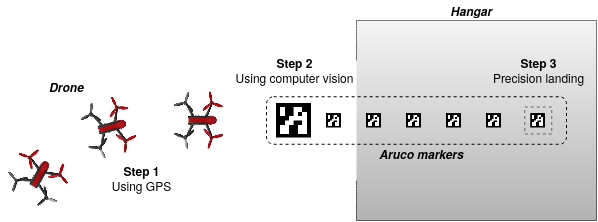
\includegraphics[height=5cm]{../Figures/masterProjectIllustration.png}
	\captionsetup{justification=centering}
    \caption{Illustration of the steps of a drone navigated autonomously using GPS to indoor navigation using computer vision leading to a precision landing }
    \label{fig:masterProjectIllustration}
\end{figure}

A solution to this problem could be to use a camera placed on the drone and analyzing the incoming data using computer vision. By placing markers on the ground, the position of these objects could be found with high precision. This would enable autonomous flight tasks where high precision of the position is needed.      

This project proposes methods for navigation in environments using computer vision. The basic idea of this can be seen in Figure \ref{fig:masterProjectIllustration}. Here the drone will fly autonomously using GPS coordinates until a higher accuracy is needed. In this case, it will be the navigation and precision landing of the drone using markers on the ground. Hence, the drone will follow the markers till a landing is required which is illustrated as step 3. The markers considered in this case will be ArUco markers, where the detection of these markers has been shown to be very accurate and reliable in changing light conditions \cite{visualmarkers}. In this example, the same marker is used for illustration, but different bit encoded ArUco markers will be used to navigate the drone to the landing sight. This is a cheap and effective solution when lack of GPS precision is present e.g using low cost GPS systems or inside buildings \cite{Visual-Inertial-Navigation}. 

The robot operating system (ROS) will be used in order to achieve autonomous flight of the drone with Gazebo as the simulation environment so that the drone can be sufficiently tested before flying. Testing of the drone will take place at Hans Christian Andersen Airport in Odense which is why the building labeled \textit{Hangar} is used in Figure \ref{fig:masterProjectIllustration}.    

\subsection{Problem Statement}

The drone must be able to fly autonomously according to ArUco markers on the ground using computer vision. This leads to the challenge of finding a robust solution for the transition of using GPS coordinates to indoor vision based navigation even in windy conditions. Furthermore, the precise landing should be implemented in such a way that the settling time, from which the drone is hovering above the marker to the landing is performed, is minimized. The same goes for the error associated with the precise landing.  

This leads to the following problems:

\begin{itemize}
    \item How can computer vision be used to detect objects?
    \item How can a smooth transition between using GPS coordinates to vision based navigation be found?
    \item How can navigation between objects be performed?
    \item How can a precise landing be executed?
    \item How can the settling time of the landing be reduced without causing instabilities to the drone?
    
\end{itemize} 

\subsection{Specification of requirements}

From the outline of the project as well as the problem statement, the following requirements for the project have been formulated:

\begin{itemize}
    \item The error of the landing must not exceed $\pm 10$ cm. 
    \item The drone should be able to make the transition of using GPS coordinates to indoor vision based navigation even in windy conditions e.g up to 8 m/s.
    \item The landing must be performed within 5 seconds from which the drone is hovering 2 meters above the landing sight to a landing is performed e.g a settling time below 5 seconds is wanted.   

\end{itemize}


\end{document}